\documentclass[onecolumn, oneside, letterpaper, draftclsnofoot, 10pt, compsoc]{IEEEtran}

\usepackage[english]{babel}
\usepackage{graphicx}
\usepackage{url}
\usepackage{setspace}
\usepackage{subcaption}

\usepackage{amssymb}
\usepackage{amsmath}
\usepackage{amsthm}
\usepackage{alltt}
\usepackage{color}
\usepackage{enumitem}
\usepackage{textcomp}
\usepackage{cite}

%\usepackage[T1]{fontenc}
\usepackage[utf8]{inputenc}
\usepackage{lmodern}
\usepackage[hidelinks]{hyperref}
\usepackage[normalem]{ulem}

\usepackage[margin=0.75in]{geometry}

% 1. Fill in these details
\def \CapstoneTeamName{         Beaver Hawks}
\def \CapstoneTeamNumber{       14}
\def \GroupMemberOne{           Anton Synytsia}
\def \GroupMemberTwo{           Matthew Phillips}
\def \GroupMemberThree{         Shanmukh Challa}
\def \GroupMemberFour{          Nathan Tan}
\def \CapstoneProjectName{      American Helicopter Society Micro Air Vehicle Competition}
\def \CapstoneSponsorCompany{   Potentially Columbia Helicopters}
\def \CapstoneSponsorPerson{    Nancy Squires}

% 2. Uncomment the appropriate line below so that the document type works
\def \DocType{Progress Report}

\newcommand{\NameSigPair}[1]{\par
\makebox[2.75in][r]{#1} \hfil   \makebox[3.25in]{\makebox[2.25in]{\hrulefill} \hfill        \makebox[.75in]{\hrulefill}}
\par\vspace{-12pt} \textit{\tiny\noindent
\makebox[2.75in]{} \hfil        \makebox[3.25in]{\makebox[2.25in][r]{Signature} \hfill  \makebox[.75in][r]{Date}}}}
% 3. If the document is not to be signed, uncomment the RENEWcommand below
%\renewcommand{\NameSigPair}[1]{#1}

%%%%%%%%%%%%%%%%%%%%%%%%%%%%%%%%%%%%%%%
\begin{document}
\begin{titlepage}
    \pagenumbering{gobble}
    \begin{singlespace}
        %\includegraphics[height=4cm]{coe_v_spot1}
        \hfill
        % 4. If you have a logo, use this includegraphics command to put it on the coversheet.
        \begin{center}
        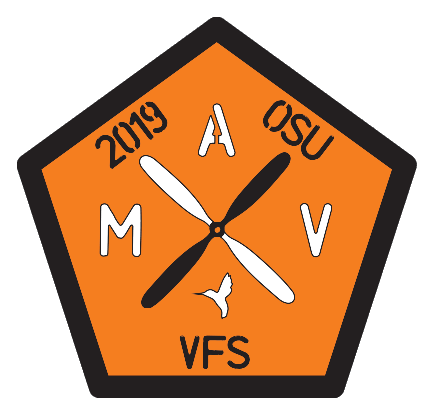
\includegraphics[height=4cm]{graphics/logo.eps}
        \end{center}
        \par\vspace{.2in}
        \centering
        \scshape{
            \huge CS Capstone \DocType \par
            {\large\today}\par
            \vspace{.5in}
            \textbf{\Huge\CapstoneProjectName}\par
            \vfill
            {\large Prepared for}\par
            \Huge \CapstoneSponsorCompany\par
            \vspace{5pt}
            {\Large\NameSigPair{\CapstoneSponsorPerson}\par}
            {\large Prepared by }\par
            Group\CapstoneTeamNumber\par
            % 5. comment out the line below this one if you do not wish to name your team
            \CapstoneTeamName\par
            \vspace{5pt}
            {\Large
                \NameSigPair{\GroupMemberOne}\par
                \NameSigPair{\GroupMemberTwo}\par
                \NameSigPair{\GroupMemberThree}\par
                \NameSigPair{\GroupMemberFour}\par
            }
            \vspace{20pt}
        }
        \begin{abstract}
        \end{abstract}
    \end{singlespace}
\end{titlepage}
\newpage
\pagenumbering{arabic}
\tableofcontents
% 7. uncomment this (if applicable). Consider adding a page break.
%\listoffigures
\listoftables
\clearpage

\section{Project Purpose}
% Talk about VFS and why they host competition

\section{Project Goals}
% MAV challenge details
% Personal Level Goals

\section{Current Project State}
% Project Design Details and Tech Review ?
% Nathan
As our project currently stands, in addition to the written documentation, we have designed a software architecture for our teams helicopter. This design takes into account a range of sensors and two cameras. Our design takes in this data on-board the Raspberry Pi, and sends the data to the appropriate place, whether that means it is sent back to the computer, or it is also used on-board the Raspberry Pi.


\subsection{Front and Bottom Video Feed}
% Nathan
A big part of this project for the Computer Science team is to deal with the cameras on the MAV. There are specific portions of the obstacle course where the pilot will have no vision of the MAV. For these parts of the course, we have a front facing camera that allows the pilot to make important decisions when piloting the MAV. The MAV design has an additional downward facing camera to assist with package pick-up. These camera feeds by design will be sent to a server run locally on a laptop, where the same laptop will display a view containing these feeds for the pilot\textquotesingle s viewing.


\subsection{Package Guidance}
% Shanmukh
% Mention bottom facing camera, image recognition. Talk about GUI and details in current project state section.
Computer Vision is an essential portion of the remote-controlled helicopter that enables the pilot to view and detect obstacles that may appear in its path. The American Helicopter Society competition contains a course with obstacles such as walls, trees, and bridges. Additionally, a part of the course cannot be seen through human eyes, so the helicopter must solely rely on a camera. Computer Vision will allow the pilot to have other intelligence data that can assist in avoiding obstacles. After exploring several image recognition APIs such as OpenCV, Amazon Recognition, and Google Cloud Vision, our team has chosen OpenCV because of the real-time image recognition benefits and it is a low-cost option.

\noindent
OpenCV, which stands for Open Computer Vision, is an open source library that gives access to numerous capabilities to efficiently detect objects. OpenCV has various inbuilt functions that allow a user to inference objects and perform actions quickly. Since OpenCV is a software development kit, the inferencing and machine learning must be performed on the local machine as there is no cloud option available. Additionally, OpenCV allows us to detect and recognize objects in real-time, so it is the chose API for our product. Specifically, we will be using OpenCV on the bottom-facing camera to find an optimal pickup point for the payload.

\subsection{Collision Warning}
% Anton
In addition to providing the pilot with video feed and package retrieval guidance, our design includes collision warning system. Collision warning system provides the pilot with awareness of the surrounding obstacles, beyond the field of view provided by the front camera. The system works in the following way. Three LV-MaxSonar ultrasonic range sensors supply the interface with instantaneous feed of obstacle detection ranges. The ranges are converted to a color scheme, ranging from green, being the farthest, to red, being the nearest. The colors are then applied to their associated semi-pie graphical user interface elements, shown in the slide. Because the pilot is not expected to look at the screen, a beeping warning sound is echoed whenever obstacles penetrate a safe radius.

One of the natural things the collision warning interface provides is the ability for the pilot to balance the aircraft in a space of obstacles. For example, whenever performing a flight through a tunnel, the pilot can focus on balancing the left and right colors within the GUI, in turn for equalizing the distances to left and right walls.

Due to potential battery power and vehicle mass limitations, our current design does not include a sensor for the rear view of the micro air vehicle. If, however, the electrical and computer engineering team, as well as the mechanical engineering team, determines that power and mass can be allocated, additional ultrasonic range sensor will be included. At the meantime, we assume the pilot restricts their maneuverability to forward and sideways.

\subsection{Collision Avoidance}
% Anton
Our stretch goal is to include collision avoidance system, where remote controls are overridden to keep the MAV at a safe distance from the obstacles. Collision avoidance is collision warning at the next level. Whenever the MAV is too close to an obstacle, the collision avoidance system overrides controls to prevent the MAV from moving further toward the obstacle. Additionally, the collision avoidance computes proper rejection pitch and roll components to ensure that the MAV does not keep moving in the direction of an obstacle.

Collision avoidance involves all the range sensors, accelerometer, and potentially the depth map from the front facing camera. For rapid response, collision avoidance is processed onboard the MAV. Displayed in the figure is a mock up how pitch and roll controls are to be overridden.

\subsection{Flight Instruments}
% Matthew
% Attidute indicator, speed indicator, height detection
% Refer to design document for details on these instruments

\section{Project Development}
% All the documents we wrote
% Nathan
So far for this project, we have written a lot of documentation in preparation for the development of the project. These documents include a problem statement, a requirements document, a technology review, a design document, and finally, this progress report.
\subsection{Problem Statement}
The problem statement helps to define the scope of our project. It introduces important definitions that help to define what our project is about and why we are doing this project.
\subsection{Requirements}
The requirements document outlines the technical scope of our project.
\subsection{Tech Review}
% Why we wrote tech reviews, but don't mention your tech
\subsection{Design}



\section{Problems and Solutions}
\subsection{Hardware Limitation}
% Hardware limitations
% Our hardware needs to fit weight limit
% Camera needs to be high resolution and be compatible with Raspberry Pi, be X frames per second

\subsection{Team Collaboration}
% Team collaboration
% Talk about how we convinced ECE and ME teams to include our bullshit

\section{Retrospective}
% Throw in your weekly progress into the associated week sections.
% We will combine them later and remove redundancy

% Also talk about collaboration with other teams

\subsection{Week 3}
\subsubsection{Anton Weekly Progress}
Progress

We have met up with one of our team members, who has already been assigned to the project before us. He introduced us to the project and showed the helicopter we will be using. We also planned a meeting time on Friday.

Problems

None

Plans

We decided to meet up on Friday with the ME leader to discuss the project and sensors we would be interested in implementing.

We also need to contact our client and determine the TA meeting times. We hope to accomplish this at the Friday's meeting.

Nathan's Weekly Progress:
\begin{itemize}
    \item Progress:

So far I have meet with my group and we have decided to communicate mainly through texting and occasionally through email. All members of the team were present and Shamukh, who has been meeting with the other subsets of the competition team, showed us the helicopter from last years competition.
    \item Problems:

Shamukh has meet with the client, Nancy, or at least that is my current understanding. But to my knowledge we have not yet designated a routine time to meet with Nancy.
    \item Plans:

October 12th will be the first time all the sub-teams will meet to discuss the project.
    \end{itemize}

\subsection{Week 4}
\subsubsection{Anton Weekly Progress}
Progress

From Tuesday through Thursday, we worked on and completed our group problem statement, utilizing the required LaTex capstone template. One of our team members will submit it today (Friday). On Wednesday, at noon, we met up with our TA, Ben. We asked Ben for insight on choosing the right kind of camera for recognition and parallax vision, as well as, the right type of ultrasonic range sensor. Luckily for us, Ben is doing a thesis on computer vision and turned our very skilled in the area of our interest. Ben guided us toward choosing the right kind of equipment for the helicopter, including Intel camera for parallax vision and reliable ultrasonic range sensor for collision avoidance. Ben as well pointed us toward his GitHub project, where we can refer to examples for our requirements document next week.

Problems

One of our team members attended the ECE group meeting and found out that they aren't planning to reserve us, the computer science team, a way for controlling the helicopter. They only have planned for providing us with feed from cameras and sensors, but not allowing us to send information to the helicopter. This seems like our work won't play a role in the competition, other than a sort of visual/collision alarm assist to the pilot. We wanted to incorporate some autonomous behavior utilizing the sensors, such as actually collision avoidance, where controls are overwritten in case the helicopter is not at a safe distance from an obstacle.

Plans

During our Friday's meeting, we discussed and prioritized all the features we would want and decided to setup a PowerPoint to present and convince the ECE team to provide us with a back-end to overwrite controls for autonomous features we are interested in implementing.


Nathan's Weekly Progress:
\begin{itemize}
    \item
    \item Progress:

This week the CS team met with the larger team to discuss the competition on Monday night. The intention was to get the list of sensors to the ECE crew, which we did. However, our client Nancy Squires was suppose to be at the meeting but never showed up.
    \item Problems:

As a CS team, we have not made contact with our client Nancy Squires, but the project needs to keep moving on. Also, one of our team members met with the larger general team today, Friday, and got the impression that feature-wise, the CS team is getting push back about implementing our ideas. With this particular project, the CS team is not necessary to compete in the competition and because there is resentment from last year's performance where automation of the helicopter went bad, the Mechanical Engineers don't want any automation, but we the CS team have ideas for a semi-automated helicopter to help the driver pilot the helicopter. Otherwise we don't have enough work to do for the rest of the year.
    \item Plans:

We are going to make a powerpoint presentation to present to the rest of the team with our ideas for the helicopter. We have 3 features that we want and need in order to actually have something to do for this competition, and one idea we are willing to part with in order to smooth over getting what we want. We will present our ideas at the next team meeting to ensure that we aren't around to just write up documents.
    \end{itemize}

Shanmukh's Weekly Progress:
\begin{itemize}
    \item Progress: We successfully opened a proper line of communication with our team. We collaborated really well with each other when working on the group problem statement, and we met twice this week to talk about our plans for developing software for the RC helicopter.
    \item Problems: There are some problems we are facing that may hinder our ability to create a software product as needed. First, we are still having trouble communicating with our client. We plan to follow up with her, or attend her office hours if she fails to respond. Secondly, we are having problems communicating with the Mechanical Engineering and Electrical Engineering majors to describe our needs. To make this project successful, we need to establish a proper line of communication so that we have the proper foundation to build our software application. And finally, our group needs to straighten a plan of attack of features to add in the RC Helicopter. Right now, we are still trying to prioritize features.
    \item Plans: We plan to establish a proper line of communication with the client and the other engineering sub-teams. Additionally, our group needs to finalize a prioritized set of features to implement for the Helicopter. We also need to begin thinking about the technical requirements for the project.
\end{itemize}

\subsection{Week 5}

\subsubsection{Anton Weekly Progress}
Progress

On Monday, during the full ME, ECE, and CS gathering, we (being the CS team) gave a presentation about the features we would like to have on the (Micro Air Vehicle) MAV and the constraints with the current, anticipated solutions to range sensors and computer vision. The ECE and ME teams gave some feedback about what is feasible and what isn't and got an idea of some things they will have to account for.

On Tuesday, we started the requirements document.

On Wednesday, we met with our TA, Ben, and found out Intel RealSense would not be feasible. Ben proposed us an alternative solution where we have 2 to 4 infrared lasers intersecting at a common point and using geometry to compute distance to target. This is a feasible solution as lasers are cheap, since they don't necessarily have to feed the user with ranges. As well, cheap high resolution camera can be found too.

Plans

We have to figure out the best way for utilizing the new camera system. We may have to have it rotate and tilt on a turret. This will allow the lasers to adjust directly to a desired target and return the most accurate distance to the target, as well as allow us to predict position and orientation of the target relative to MAV. We plan on meeting with our team next week to discuss the new system.

We additionally have to complete the requirements document, during the weekend, and research the components we would need for the MAV. This will aide us in researching the type of components for the upcoming individual assignment.

Problems

The MEs are not entirely for the aspect of having moving parts on board. We will have to figure out how to keep the entire system stable as the camera turret rotates. We additionally figured ultrasonic range sensors have limits to the objects they can detect. We may have to use a combination of ultrasonic and infrared obstacle detection sensors to develop a reliable collision avoidance system.


Nathan's Weekly Progress:
\begin{itemize}
    \item Progress:

This week the focus of our resources have been working on getting our list of desired sensors to the rest of the team as a whole.

Overall we are about half way through having all of the sensors we want figured out.
    \item Progress:

This week the focus of our resources have been working on getting our list of desired sensors to the rest of the team as a whole.

Overall we are about half way through having all of the sensors we want figured out.
    \item Plans:

For next week we need to finish up our requirements doc as well as get specific senors chosen for our project. Our TA Ben will be a big help with this in making sure our sensors are realistic.
    \end{itemize}
Shanmukh's Weekly Progress:
\begin{itemize}
    \item Progress: Our group had an in-depth discussion with our client and we talked about the possibilities of implementing computer vision and sensor intelligence to benefit the helicopter. Additionally, we made sure the mechanical engineers and ECEs knew of our plans.
    \item Problems: Some of the tools that we wanted to use did not meet the requirements of the helicopter. They were either too heavy or they required too much bandwidth to transmit data, which would drain the battery life of the aircraft.
    \item Plans: As a group, we want to make sure we choose tools so that they meet our aircraft weight and battery requirements.
\end{itemize}


\subsection{Week 6}

\subsubsection{Anton Weekly Progress}
Progress

On Monday and Tuesday we were working hard toward completing and compiling our requirements document. On Wednesday, we met with our TA to review our requirements document, as well as, get additional insight regarding infrared laser distance sensing. Ben suggested us to use the SparkFun depth camera as a simpler, but a more viable solution. That same day, we went to ECEs meeting regarding the depth camera, which can also do color vision. They said, it has a good cost and voltage I/O requirements but because it uses USB3.0, they will not be able to implement it. So, we'll have to use simple technologies, like lasers and cameras or discard the idea of lasers altogether.

Problems

We still have to decide the parts and cameras. The individual research will help us pinpoint the technologies.

Plans

On Friday, we intend to do our individual research. On Monday, we intend to meet up and put together a presentation of our findings to present during ECEs and MEs meeting at 7:30pm.

Nathan's Weekly Progress:
\begin{itemize}
    \item Progress:

We have finished a first draft for our requirements document and we have received some feedback for another substitution. In terms of our requirements document, our TA Ben had some formatting points for us to clean up, as well as a restructure of our Gantt chart. In addition to these changes, the content of our requirements document will later change because our goals in terms of the project aren't completely set in stone yet and we are currently working on deciding what kind of sensors will best for our team. While we haven't finalized our ideas, we just submitted some individual tech reviews which we will later add together.
    \item Problems:

Choosing a camera for the bottom and front sides of our camera is not easy. There are weight, power, and quality requirements. Additionally we have an overall budget of 3000 to stick to, but that will be less of an issue, especially with the size of the camera. Also, if our camera is strong enough we won't need extra infrared lasers on the the from of the camera to calculate distance, however stronger cameras like this typically don't connect well with the Arduino that the ECE side of our team wants to use.
    \item Plans:

In terms of writing assignments for the capstone class, our work load looks lighter this upcoming week. This will give us more time to research our sensors so we can get that finalized for the rest of our team. Additionally, we may work more on tidying up our documents.
    \end{itemize}
Shanmukh's Weekly Progress:
\begin{itemize}
    \item Progress: This week, my team and I were proactive in meetings with the mechanical engineering and computer engineering subteams. We made sure the subteams understood our technical requirements to implement computer vision technology on the helicopter. In addition, we discussed in detail about our team standards and what we expect from each other.
    \item Problems: My team and I did not have any problems this week. However, most of the team members, including myself got sick, stressed out from midterms and had job interviews to do/prepare for so we all didn't have a chance to sit out and update each other on our progress.
    \item Plans: While my group and I had a busy week, the next week should be tamer. We are planning to spend more time with each other to finalize our technical requirements and discuss plans to start implementing the software.
\end{itemize}


\subsection{Week 7}

\subsubsection{Anton Weekly Progress}
Progress

We did one presentation on Monday regarding the ultrasonic sensors and the types to utilize for down, front, and side directions. We have also discussed a few depth perception cameras with our TA, Ben, on Wednesday. Throught the week we were working on our individual tech reviews.

Problems

The ECEs decided their original chosen board, Arduino AT Mega, may be unsuitable for doing high resolution video streaming at at least 15 fps. Rather than figuring out how to compress the video, the ECEs decided they will stitch to Raspberry Pi. This is good for us as we have a greater potential to utilize computationally expensive operations onboard and its bad for ECEs, as part of their requirement is to deal with registers if I have understood them correctly.

Plans

Today, Friday, the plan is to revise our tech reviews so that we can focus on design document in the future (in addition to getting a fine grade). Next week we will have to meet up with the ECE team to discuss our and theirs chosen tech and how they and we will implement it. This will narrow us closer to having a plan for the what and the how of the project.


Nathan's Weekly Progress:
\begin{itemize}
    \item Progress:

This week I attended the weekly team meeting and finished up the final draft for the tech review. I also meet with the TA, Ben, to discuss the next upcoming assignment.
    \item Problems:

No outstanding problems this week.
    \item Plans:

Next week we start our design document which will outline how we will attack our project.
    \end{itemize}
Shanmukh's Weekly Progress:
\begin{itemize}
    \item Progress: Our team and I made good progress by discussing our technology reviews. We made sure that every team member was an expert on the topics they chose to write about. Additionally, we solidified our plans with the electrical and mechanical engineers so they could get the hardware portions running.
    \item Problems: The only problem we faced this week was an inconsistent timeline for the hardware to be set up with the raspberry so that we can start implementing the software features of the project. However, we can make a proper plan with the electrical engineering team to figure this out.
    \item Plans: Our plan for next week is to set a plan with the electrical engineers so we can help purchase our sensors and cameras to be set up on the raspberry pi. Also, we will be working with them to get a proper feed for the sensor and visual data so the computer science team can begin developing software features.
\end{itemize}


\subsection{Week 8}

\subsubsection{Anton Weekly Progress}
Progress

On Wednesday, Shanmukh, I, the mechanical team, and one representative from the electrical presented our plan to our sponsor, Anna Royce. Shanmuckh talked about image recognition for helipad guidance and I talked about collision warning and collision avoidance with ultrasonic range sensors. The presentation was primarily focused on the mechanical team to explain their design and how it is going to be different from the last year's design. There was not much input from the computer science team (us) or the electrical team. The other two members of the CS team, Matthew and Nathan, were at the TA meeting discussing the design process. On Thursday, we met up to start working on our design and to unite our ideas. We did another meeting on Friday to continue the meeting.

Problems

None

Plans

We planned to meet up on Saturday for further discussion of our design. The idea is to have our design ideas and goals finalized before the Monday's meeting with the ECE and ME teams. We will present it to them and have them evaluate our decisions.


Nathan's Weekly Progress:
\begin{itemize}
    \item Progress:

So far we have meet with our TA to discuss the design document and we have started designing the software architecture for the competition. We have done some block diagrams and flow diagrams on white board to describe the composure of our systems, both for the helicopter and the GUI application to display the camera feed from the helicopter.
    \item Problems:

Finding to meet is always a problem with the teams varying schedules. For this document we need to meet more than usual to discuss the actual design before we can start writing the design document. Another problem is organization of the current designs we have. At the moment all the designs are saved as photos on my phone and I  need to upload them to our slack channel and eventually our GitHub.
    \item Plans:

Our team will continue to meet and discuss our design until we have it mostly figured out, at which point we will be able to easily separate and draft separate parts of the design document. We also need make a plan of what and how we are going to show the Mechanical and Electrical portions of our team to get their feedback to make sure they are okay with our design.
    \end{itemize}
Shanmukh's Weekly Progress:
\begin{itemize}
    \item Progress: This week, my team and I made a concrete plan in order to tackle the design document by discussing all the components of the product. Additionally, we divided tasks and will begin drafting our document once we discuss our plans at the large team meeting which is comprised of the mechanical engineers, electrical engineers, and our client.
    \item Problems: We did not face any problems this week. However, we may need to revise our design plan after meeting with our client and the electrical engineering team.
    \item Plans: Our plan for next week is to pitch our design to the large team and make any revisions as necessary. Once we finalize our plan, we will begin writing our sections of the document and will be ready to submit it by next Tuesday.
\end{itemize}


\subsection{Week 9}

\subsubsection{Anton Weekly Progress}
Progress

Monday's meeting with ECE and ME teams was reassuring a way that it allowed us to see that all our design plans and ideas are coming together. The ME team presented their helicopter design and the plan for implementing components and sensors. Their solution for the helicopter design is very light weight and the helicopter itself can lift 1000 grams. This means we are not limited when it comes to mass restrictions other than having to stick with the 500 gram mass limit. The ECE team presented their plan for utilizing Raspberry Pi 0. From our side, Nathan gave a brief presentation regarding our onboard system architecture. This was meant for the ECEs team to analyze our plans and provide feedback regarding the feasibility. We, as well, received reassurance from the ECE team on ordering the Eyes3d depth camera for our tront-facing camera. They already have ordered the down facing camera. Regarding the range sensors, the ECE team said they will send us an email on whether to order 4 LV-MaxSonar sensors. At the moment we are awaiting for their response.

Problems

None

Plans

The objective is to work on the design document throughout the week and the weekend. Our TA, Ben, provided us with information on generating UML diagrams for the design document, so we have the resources we need to complete the task. We plan to meet up on Tuesday to finish the design document.


Nathan's Weekly Progress:
\begin{itemize}
    \item Progress:
    This past week we finished the high level design of our system and have started documenting our design. This design has been shared with the larger team.
    \item Problems:
    The design document needs to be finished and we have a holiday blocker this weekend.
    \item Plans:
    Finish the design document and start cleaning up the rest of the documents.
    \end{itemize}
Shanmukh's Weekly Progress:
\begin{itemize}
    \item Progress: Because of the short week, we were not able to meet as a team to discuss the design document in depth. Thanks to our early planning, we were able to divide tasks and iron out complexities last week. Additionally, we have begun working on our individual components for the design document and we found a UML diagram generator to use.
    \item Problems: We did not face any problems this week since we had in-depth discussions on our document last week. We are continuing to work on our individual components.
    \item Plans: Our plan is to finish our portions of the design document by Monday so we can email our UML diagrams to our TA for approval. We are also planning to meet on Tuesday as a group to put all our parts together for a final review of the document before submitting it on Tuesday night.
\end{itemize}


\clearpage
\medskip
\bibliographystyle{IEEEtran}
\bibliography{ref}
\end{document}